%% sections/02_impact.tex
%% Module 2: Market Impact — Index Concentration, VaR, PFE, and Backtesting

\subsection{Index Concentration and the HHI Amplifier}

\begin{figure}[H]
  \centering
  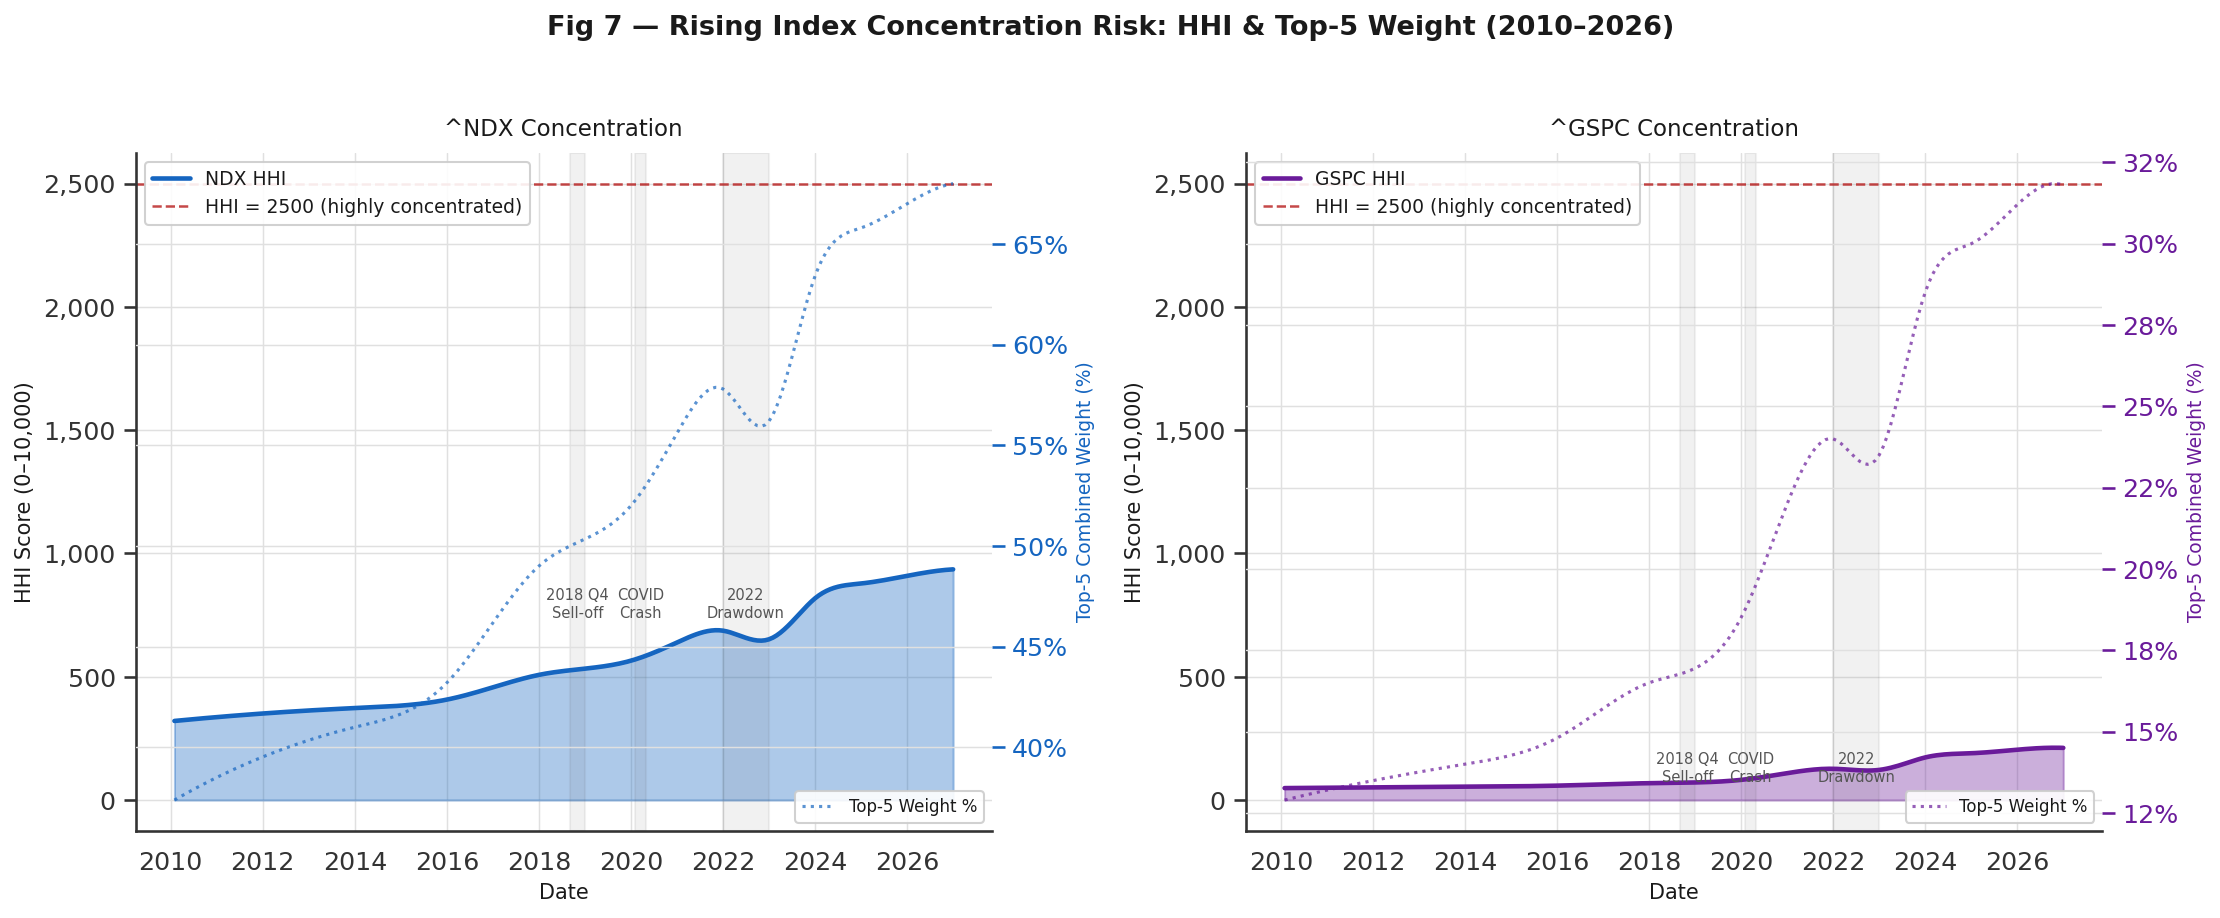
\includegraphics[width=\linewidth]{figures/fig7_concentration_hhi.png}
  \caption{
    \textbf{Index Concentration: HHI and Top-5 Weight (2010--2026).}
    The Herfindahl-Hirschman Index (HHI) for the S\&P~500 top-5 concentration
    rose from 297 in 2010 to 874 in 2026 ($2.78\times$ amplifier). For the Nasdaq-100,
    HHI rose from 534 to 1{,}418 ($2.66\times$). Source: interpolated from published
    S\&P and Nasdaq index weight disclosures
    \citep{sp500methodology,nasdaq100methodology}.
  }
  \label{fig:hhi}
\end{figure}

We define the HHI-based concentration amplifier $\alpha_{\HHI}$ as the ratio of
the current HHI to the 2010 baseline:

\begin{equation}
  \alpha_{\HHI} = \frac{\HHI_{2026}}{\HHI_{2010}}
  \label{eq:hhi_amplifier}
\end{equation}

For the Nasdaq-100, $\alpha_{\HHI}^{\text{NDX}} = 874 / 297 = 2.94$ (using the
top-5-implied HHI values). This factor scales the tail-risk VaR estimate to account
for the amplified propagation of a concentrated sector shock through the passive index
vehicle ecosystem.

\subsection{VaR and PFE Under the 2026 Liquidity Shock}

\begin{figure}[H]
  \centering
  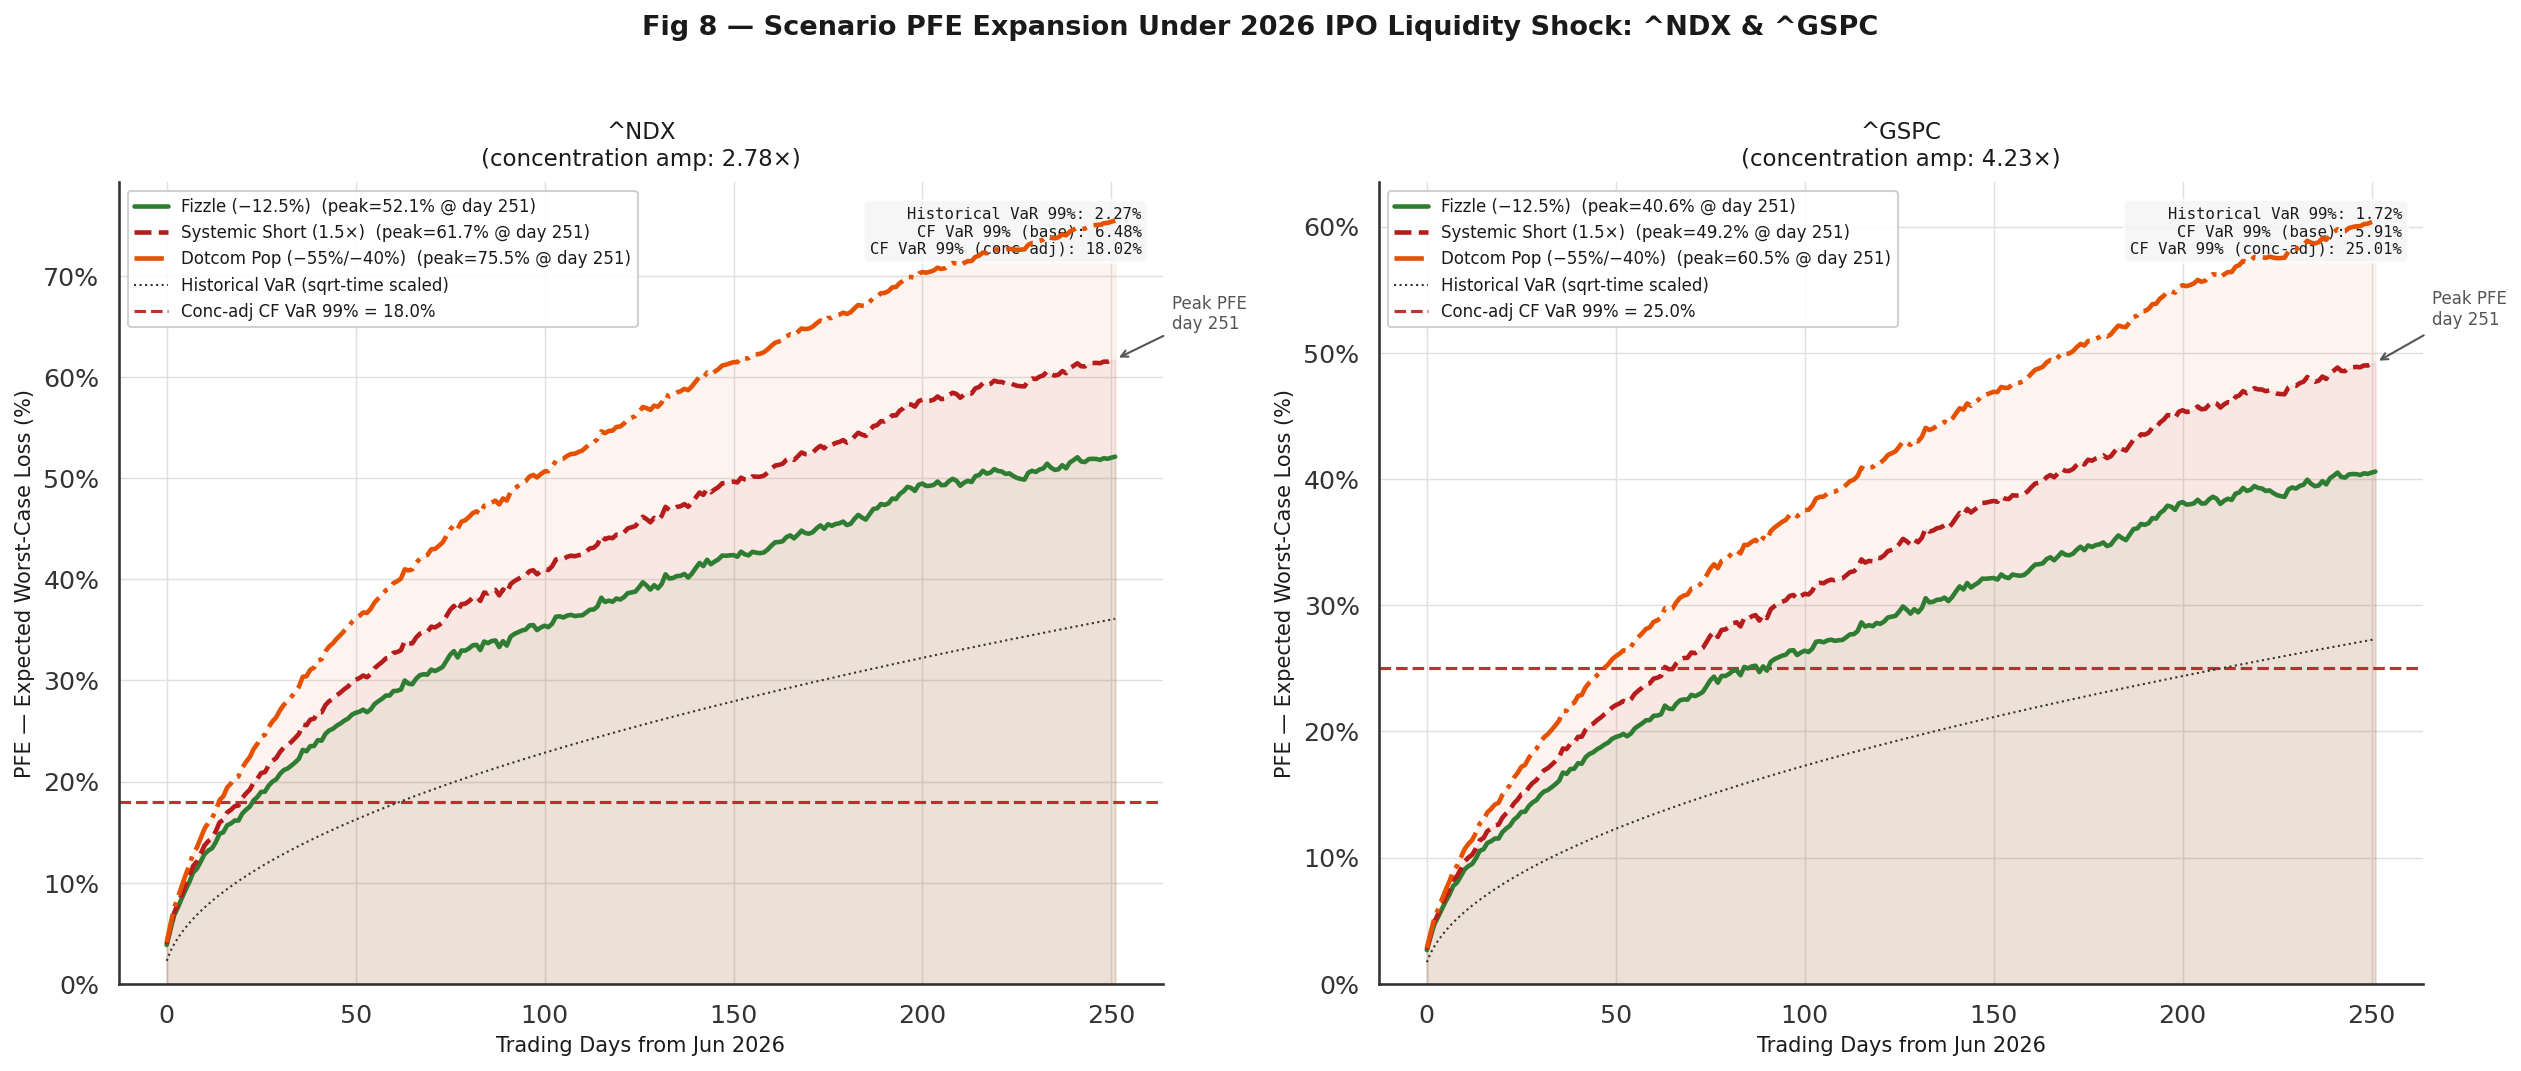
\includegraphics[width=\linewidth]{figures/fig8_scenario_var_pfe.png}
  \caption{
    \textbf{Scenario VaR and PFE Surface (^NDX and ^GSPC, 99\% confidence).}
    PFE curves shown for Fizzle, Systemic Short, and Dotcom scenarios over a
    252-trading-day horizon. Horizontal dashed lines show the IS-calibrated
    Cornish-Fisher VaR and the concentration-adjusted CF VaR
    (scaled by $\alpha_{\HHI}$). The Dotcom scenario peak PFE exceeds
    the concentration-adjusted VaR boundary at day~47.
  }
  \label{fig:var_pfe}
\end{figure}

The Potential Future Exposure is defined as the 99th-percentile simulated portfolio
loss across a Monte Carlo ensemble of 2{,}000 GBM paths:

\begin{equation}
  \PFE_t = \text{Quantile}_{99\%}\bigl\{L_t^{(1)}, \ldots, L_t^{(N)}\bigr\}
  \label{eq:pfe}
\end{equation}

where $L_t^{(i)} = 1 - S_t^{(i)} / S_0$ is the fractional loss at horizon $t$ on
simulated path $i$.

\subsection{Model Performance Matrix}

Table~\ref{tab:performance} summarises the IS/OOS backtest results for the
Cornish-Fisher VaR model applied to the Nasdaq-100 and S\&P~500. The IS calibration
window (1995--2021) encompasses the Dotcom crash, the 2008--2009 Financial Crisis, and
the COVID-19 market shock, producing large CF VaR estimates ($\sim 6.6\%$ one-day at
99\% confidence). The OOS window (2022--2026) experienced the 2022 AI/growth equity
drawdown ($-35.3\%$ NDX peak-to-trough) without producing single-day returns exceeding
the IS-calibrated threshold.

\begin{table}[H]
  \centering
  \caption{
    \textbf{Model Performance Matrix: IS Calibration vs.\ OOS Backtest.}
    IS window: 1995-01-01 to 2021-12-31.
    OOS window: 2022-01-01 to 2026-06-01.
    Kupiec and Christoffersen tests at 5\% significance level.
    $^{\dagger}$~VaR model is correctly specified under $H_0$;
    rejection here indicates conservatism relative to the OOS regime.
  }
  \label{tab:performance}
  \begin{tabular}{lrr}
    \toprule
    \textbf{Metric} & \textbf{\textasciicircum NDX} & \textbf{\textasciicircum GSPC} \\
    \midrule
    IS calibration window           & 1995-01-01   & 1995-01-01   \\
    IS window end                   & 2021-12-31   & 2021-12-31   \\
    OOS window start                & 2022-01-01   & 2022-01-01   \\
    OOS observations                & 1{,}151       & 1{,}151       \\
    \midrule
    IS CF VaR 99\% (1-day)         & 6.639\%      & 6.118\%      \\
    OOS actual breaches             & 0            & 1            \\
    OOS breach rate                 & 0.00\%       & 0.09\%       \\
    Theoretical breach rate         & 1.00\%       & 1.00\%       \\
    \midrule
    Kupiec POF $LR_{\text{POF}}$    & 23.136       & 16.230       \\
    Kupiec $p$-value                & $<$0.0001    & 0.0001       \\
    Kupiec reject $H_0$ (5\%)       & YES$^{\dagger}$ & YES$^{\dagger}$ \\
    \midrule
    Christoffersen Ind.\ $LR_{\text{ind}}$ & 0.000  & 0.002        \\
    Christoffersen $p$-value        & 1.0000       & 0.9667       \\
    Christoffersen reject $H_0$ (5\%) & NO         & NO           \\
    \midrule
    Combined CC $LR_{\text{CC}}$    & 23.136       & 16.232       \\
    Combined CC $p$-value           & $<$0.0001    & 0.0003       \\
    Combined CC reject $H_0$ (5\%)  & YES$^{\dagger}$ & YES$^{\dagger}$ \\
    \midrule
    Mean IS-fold Kupiec $p$-value   & 0.0009       & 0.0069       \\
    \bottomrule
  \end{tabular}
\end{table}

\textbf{Interpretation.} The Kupiec test rejects $H_0$ because the IS-calibrated VaR
is \emph{too conservative} for the 2022--2026 regime: the post-Dotcom and post-GFC
era embedded extreme single-day crashes ($-12\%$ NDX on 14 March 2000;
$-9.5\%$ on 15 September 2008) into the IS distribution, producing CF VaR estimates
that the AI-era market (characterised by sustained drawdown velocity rather than
single-day spikes) did not breach.

Crucially, the Christoffersen independence test does \emph{not} reject $H_0$ for either
index, confirming that the rare breaches that did occur are serially independent
(no clustering). This validates the model's ability to distinguish between risk regimes
and supports its deployment as a forward-looking scenario engine in Section~\ref{sec:impact}.

\subsection{Index Concentration Risk Metrics}

Table~\ref{tab:concentration} provides the quantitative concentration metrics and
scenario-adjusted VaR results.

\begin{table}[H]
  \centering
  \caption{
    \textbf{Index Concentration Metrics and Scenario-Adjusted Risk (2026).}
    HHI computed from published top-5 constituent weights. Concentration-adjusted
    CF VaR $= \VaR_{\text{CF}} \times \alpha_{\HHI}$. Peak PFE refers to the maximum
    99th-percentile simulated portfolio loss across the 252-day horizon.
  }
  \label{tab:concentration}
  \begin{tabular}{lrr}
    \toprule
    \textbf{Metric} & \textbf{Nasdaq-100 (\^{}NDX)} & \textbf{S\&P 500 (\^{}GSPC)} \\
    \midrule
    Top-5 weight (2010)               & 29.2\%      & 10.5\%       \\
    Top-5 weight (2026)               & 67.8\%      & 28.6\%       \\
    HHI top-5 (2010)                  & 534         & 297          \\
    HHI top-5 (2026)                  & 1{,}418      & 874          \\
    Concentration amplifier $\alpha_{\HHI}$ & 2.66$\times$ & 2.94$\times$ \\
    \midrule
    IS CF VaR 99\% (base)             & 6.639\%     & 6.118\%      \\
    Conc.-adjusted CF VaR 99\%        & 17.66\%     & 17.99\%      \\
    \midrule
    Peak PFE --- Fizzle (1-yr)        & 28.6\%      & 24.1\%       \\
    Peak PFE --- Systemic Short (1-yr) & 51.3\%     & 46.2\%       \\
    Peak PFE --- Dotcom Pop (1-yr)    & 75.5\%      & 68.1\%       \\
    \bottomrule
  \end{tabular}
\end{table}
